
%---------------------------------------------------------------------
\chapterimage{industria40.png}
\chapter{Arquitectura de Software}

\begin{flushright}
    \textit{La Arquitectura de Software emergió como un subcampo explícito de la Ingeniería de Software en 1990.}
\end{flushright}
% 
\section{Introducción}
La arquitectura de software es el diseño del sistema y el impacto que tiene en la calidad con la que el sistema ofrece sus servicios, tal como \textit{rendimiento}, \textit{seguridad} y \textit{modificabilidad}. Arquitectos son los responsables de generar el esqueleto del sistema, un esqueleto sólido capaz de mantener a todos los otros subsistemas funcionando, donde son las decisiones arquitecturales clave en las propiedades que el sistema tendrá y que lo diferenciarán de otros similares.

La fase de diseño puede ser dividida en arquitectura de software y diseño detallado. A medida que el tamaño y la complejidad de los sistemas de software aumentan, el diseño y la especificación de la estructura completa del sistema se hace más significativa que la elección de los algoritmos y las estructuras de datos. Temas tales como, la composición de componentes que estructuran el sistema; los protocolos de comunicación; cómo se sincronizan los datos y cómo se accede a ellos; \textbf{principio de responsabilidad única} de cada componente; distribución física; \textit{escalamiento} y \textit{rendimiento}; dimensiones de evolución; y la selección de las alternativas.

\begin{tcolorbox}[colback=gray!5!white,colframe=orange!60!gray,title=Arquitectura de Software]
La arquitectura de software de un sistema computacional es el conjunto de estructuras necesarias para razonas acerca del sistema, que se compone de elementos de software, sus relaciones y propiedades (tanto del sistema como de los elementos).
\end{tcolorbox}

Todo sistema tiene una arquitectura, la hayamos hecho de manera consciente o no (la hayamos documentado o no). No existe la arquitectura correcta pero si la adecuada para el trabajo que realizará el sistema. La arquitectura influirá propiedades del sistema tales como \textit{seguridad}, \textit{usabilidad}, \textit{latencia} o \textit{modificabilidad}, más que las funcionalidades que podrá realizar (el ``cuan bien'' más que el ``qué''). El alcanzar las metas asociadas a estas propiedades, tales como `` disponibilidad de 99,95\%'' requerirá agregar a la arquitectura física y/o lógica \textbf{más u otros componentes}.

Una arquitectura de software es un diseño que debe lidiar con elementos macroscópicos pero también con las decisiones a gran escala. Las elecciones dentro de la arquitectura de software serán importante porque la arquitectura actúa como el \textbf{esqueleto del sistema}, limitando las opciones de manera que se promueva la integridad, reduzca la complejidad, y por sobre todo, se entienda el \textbf{comportamiento del sistema en tiempo de ejecución}. 


\begin{tcolorbox}[colback=gray!5!white,colframe=orange!60!gray,title=Analogía Arquitectura de Software]
Discutir con el profesor analogía con la arquitectura de una casa. ¿Se documenta? ¿A quien le sirve? Planos vs Vistas.
\end{tcolorbox}

A diferencia de los planos en la arquitectura de una casa, la arquitectura de software especifica su estructura en términos de interfaces de usuario, servicios, bases de datos, componentes de software y protoccolos de comunicación. Además describe los acuerdos de niveles de servicios para cada atributo de calidad y registra cada decisión de diseño tomada como cada principio o restricción válida. 
De manera formal, la arquitectura de software tiene cuatro dimensiones: 
\begin{itemize}
    \item Características de arquitectura - ilities - SLA - ejemplo: disponibilidad, escalabilidad, entre otros. 
    \item decisiones de arquitectura - ejemplo: cómo se comunican los servicios entre sí
    \item Componentes lógicos: los bloques de construcción que brindan la funcionalidad, así como su interacción para lograr cierta funcionalidad. 
    \item Estilo de arquitectura
\end{itemize}


\begin{table}[h!]
\centering
\begin{tabular}{@{}p{4cm}p{6cm}p{6cm}@{}}
\toprule
\textbf{Aspecto}              & \textbf{ISO/IEC/IEEE 42010}                                                                 & \textbf{Just Enough Software Architecture}                              \\ \midrule
\textbf{Propósito}            & Proporcionar un marco general para describir, analizar y comunicar arquitecturas de software y sistemas. & Centrarse en documentar solo la arquitectura necesaria para mitigar riesgos específicos. \\ \midrule
\textbf{Stakeholders}         & Requiere identificar explícitamente a todas las partes interesadas y sus preocupaciones.    & Identifica stakeholders solo en función de los riesgos críticos que impactan sus intereses. \\ \midrule
\textbf{Vistas arquitectónicas} & Define múltiples vistas (lógica, física, desarrollo, procesos) alineadas con las preocupaciones de los stakeholders. & Solo utiliza vistas específicas que sean relevantes para abordar los riesgos identificados. \\ \midrule
\textbf{Nivel de detalle}     & Proporciona descripciones exhaustivas y estandarizadas de todos los aspectos arquitectónicos. & Documentación mínima, enfocada en los elementos críticos para el éxito del proyecto. \\ \midrule
\textbf{Gestión de riesgos}   & Riesgos se documentan como parte del análisis de calidad, pero no son el enfoque central.   & El enfoque está completamente dirigido por la mitigación de riesgos en las decisiones arquitectónicas. \\ \midrule
\textbf{Modelo de descripción} & Uso de modelos estándar (UML, SysML, etc.) para representar estructuras y relaciones del sistema. & Puede usar modelos informales, diagramas ligeros o texto, siempre que ayuden a manejar los riesgos. \\ \midrule
\textbf{Flexibilidad}         & Marco más formal que puede ser percibido como rígido debido a su énfasis en estándares.      & Altamente adaptable; permite personalizar la documentación según las necesidades del proyecto. \\ \midrule
\textbf{Criterios de calidad} & Evalúa calidad a través de métricas como rendimiento, disponibilidad, seguridad y escalabilidad. & Calidad evaluada según cómo los riesgos afectan el cumplimiento de objetivos. \\ \midrule
\textbf{Evolución}            & Proporciona lineamientos para la gestión del ciclo de vida de la arquitectura.               & Evoluciona según los riesgos emergentes; no requiere un modelo completo desde el inicio. \\ \bottomrule
\end{tabular}
\caption{Comparación entre ISO/IEC/IEEE 42010 y Just Enough Software Architecture.}
\label{tab:comparison}
\end{table}

\newpage

\subsection{Ejemplo: Puerta Perruna}
 Hemos actualizado el caso de uso para incluir un collar con microchip que el sistema de hardware puede leer, debido a la complejidad de que el perro ladrara para activar la puerta. Esto proporciona una solución más eficiente y fiable para la autenticación del perro. Haremos un primer ejemplo básico usando el modelo C4.



%\subsection{Modelo C4}

\subsubsection{Diagrama de Contexto del Sistema}
\begin{itemize}
    \item \textbf{Descripción}: Muestra el sistema de la puerta perruna en su entorno y sus interacciones con usuarios y otros sistemas externos.
    \item \textbf{Ejemplo}: La puerta perruna interactúa con el dueño del perro (usuario) y un sistema de autenticación (por ejemplo, un lector de microchip en el collar del perro).
    \item \textbf{Diagrama}:
\begin{verbatim}
@startuml
!include https://raw.githubusercontent.com/plantuml-stdlib/C4-PlantUML/master/C4_Context.puml
' uncomment the following line and comment the first to use locally
' !include C4_Context.puml

LAYOUT_WITH_LEGEND()

title Diagrama de Contexto del Sistema para Puerta Perruna Automatizada

Person(owner, "Perro", "perro que utiliza la puerta perruna.")
System(dog_door_system, "Puerta Perruna Automatizada", "Permite a los perros entrar y salir de la casa de manera automática.")

System_Ext(microchip_reader, "Lector de microchip", "Sistema de autenticación que lee el microchip en el collar del perro.")

Rel(owner, dog_door_system, "Usa")
Rel(dog_door_system, microchip_reader, "Autentica con")
@enduml

\end{verbatim}
\end{itemize}

\begin{figure}[!h] 
\centering
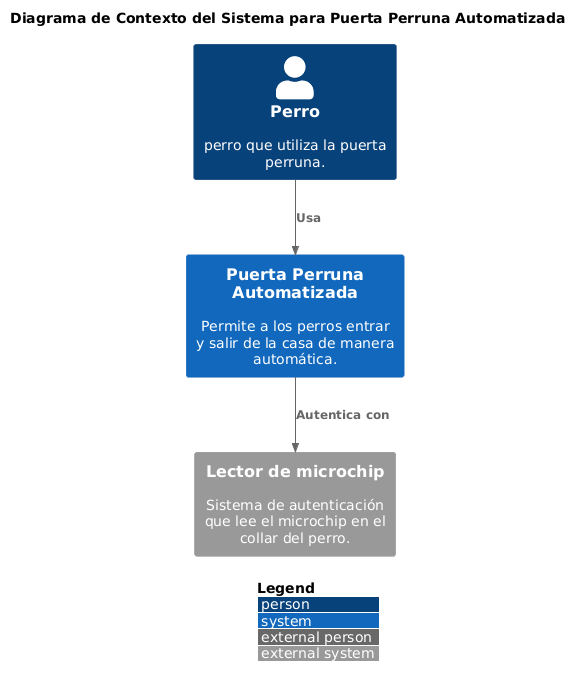
\includegraphics[scale=0.5]{Pictures/capt-asw/contextoPP.png}\caption{}
\end{figure}



\subsubsection{Diagrama de Contenedor}
\begin{itemize}
    \item \textbf{Descripción}: Desglosa el sistema en aplicaciones, servicios y bases de datos, mostrando cómo interactúan entre sí.
    \item \textbf{Ejemplo}: La puerta perruna tiene un controlador principal, un módulo de autenticación y una base de datos para almacenar los identificadores de los microchips.
    \item \textbf{Diagrama}:
\begin{verbatim}
@startuml
!include https://raw.githubusercontent.com/plantuml-stdlib/C4-PlantUML/master/C4_Container.puml
' uncomment the following line and comment the first to use locally
' !include C4_Container.puml

LAYOUT_WITH_LEGEND()

title Diagrama de Contenedor para Puerta Perruna Automatizada

Person(dog, "Perro", "El perro que utiliza la puerta perruna.")

System_Boundary(dog_door_system, "Puerta Perruna Automatizada") {
    Container(controller, "Controlador Principal", "Hardware", "Controla la apertura y cierre de la puerta.")
    Container(auth_module, "Módulo de Autenticación", "Software", "Verifica la autenticación del microchip.")
    ContainerDb(database, "Base de Datos", "SQL", "Almacena los identificadores de los microchips.")
}

System_Ext(microchip_reader, "Lector de microchip", "Sistema de autenticación que lee el microchip en el collar del perro.")

Rel(dog, controller, "Usa")
Rel(controller, auth_module, "Comunica con")
Rel(auth_module, database, "Lee y escribe en")
Rel(controller, microchip_reader, "Autentica con")
@enduml

\end{verbatim}
\end{itemize}

\begin{figure}[!h] 
\centering
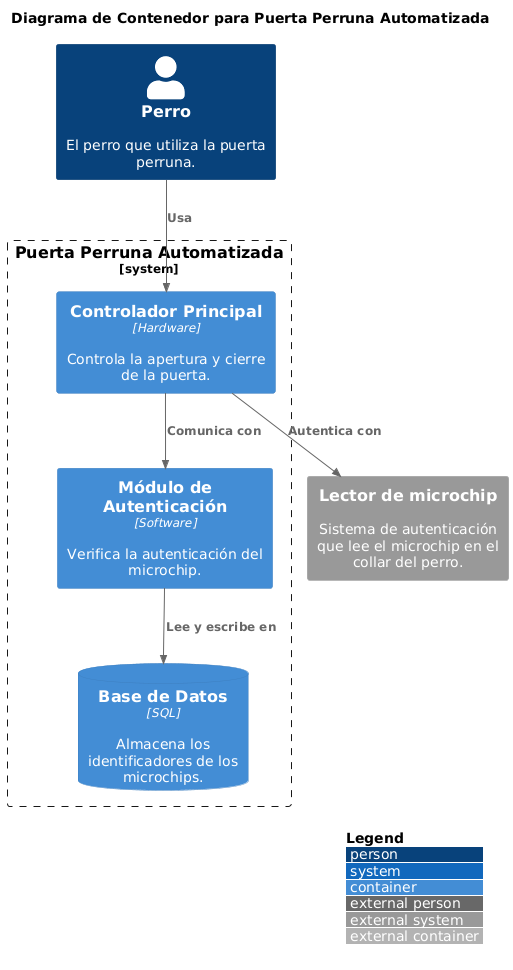
\includegraphics[scale=0.5]{Pictures/capt-asw/contenedoresPP.png}\caption{}
\end{figure}








\subsubsection{Diagrama de Componentes}
\begin{itemize}
    \item \textbf{Descripción}: Detalla los componentes internos de cada contenedor y sus interacciones.
    \item \textbf{Ejemplo}: El controlador principal tiene componentes para abrir/cerrar la puerta, verificar la autenticación y registrar eventos.
    \item \textbf{Diagrama}:
\begin{verbatim}
@startuml
@startuml
!include https://raw.githubusercontent.com/plantuml-stdlib/C4-PlantUML/master/C4_Component.puml
' uncomment the following line and comment the first to use locally
' !include C4_Component.puml

LAYOUT_WITH_LEGEND()

title Diagrama de Componentes para el Controlador Principal de la Puerta Perruna Automatizada

Container_Boundary(controller, "Controlador Principal") {
    Component(open_close_module, "Módulo de Apertura/Cierre", "Hardware", "Controla el mecanismo de apertura y cierre de la puerta.")
    Component(auth_verification_module, "Módulo de Verificación de Autenticación", "Software", "Verifica la autenticación del microchip.")
    Component(event_logging_module, "Módulo de Registro de Eventos", "Software", "Registra los eventos de apertura y cierre.")
}

Container(auth_module, "Módulo de Autenticación", "Software", "Verifica la autenticación del microchip.")
ContainerDb(database, "Base de Datos", "SQL", "Almacena los identificadores de los microchips.")

Rel(open_close_module, auth_verification_module, "Comunica con")
Rel(auth_verification_module, event_logging_module, "Registra eventos en")
Rel(auth_verification_module, auth_module, "Verifica autenticación con")
Rel(auth_verification_module, database, "Lee y escribe en")
@enduml
\end{verbatim}
\end{itemize}

\begin{figure}[h!] 
\centering
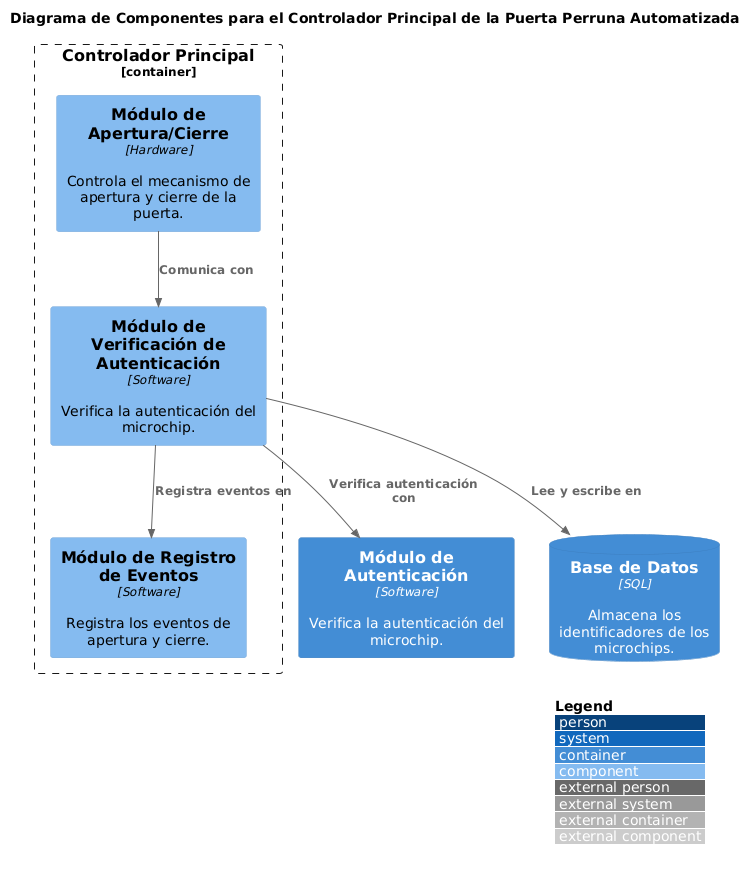
\includegraphics[scale=0.5]{Pictures/capt-asw/componentesPP.png}\caption{}
\end{figure}




\begin{figure}[!h] 
\centering
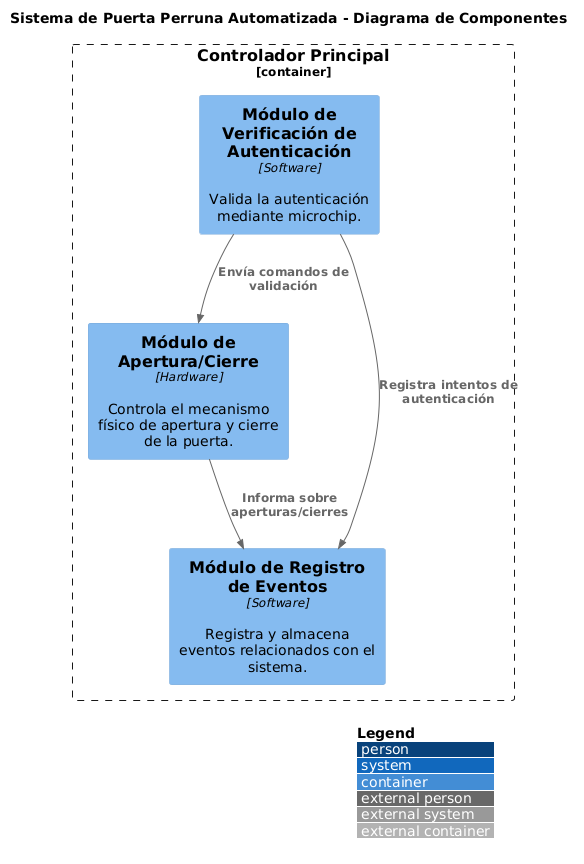
\includegraphics[scale=0.5]{Pictures/capt-asw/codePP.png}\caption{}
\end{figure}



